\documentclass[12pt, A4paper]{article}
\usepackage{hyperref}
\usepackage{booktabs}
\usepackage{graphicx}
\usepackage{amsmath}
\usepackage[utf8]{inputenc} 
\usepackage{pdflscape}

\usepackage{mhchem}
\usepackage[numbers]{natbib}

\usepackage{fancybox}
\usepackage{graphicx}
\usepackage{color}
%\usepackage[margin=0.7in]{geometry}
\setlength{\abovetopsep}{1em}

\usepackage{siunitx}
\sisetup{locale=ZA}


\usepackage[margin=1.2in]{geometry}

\graphicspath{{graph/}}

\title{CIR310 Phase equilibrium project\\Part 2}
\date{Submission deadline: 24.04.2017 before 13:30}

\newcounter{eqs}
\setcounter{eqs}{0}
\newcommand{\eq}{\stepcounter{eqs}\arabic{eqs}}

\newcounter{variables}
\setcounter{variables}{0}

\newcounter{inputs}
\setcounter{inputs}{0}
\newcommand{\definput}[1]{\ensuremath{#1}\stepcounter{inputs}\stepcounter{variables}}

\newcounter{outputs}
\setcounter{outputs}{0}
\newcommand{\defoutput}[1]{\ensuremath{#1}\stepcounter{outputs}\stepcounter{variables}}

\newcounter{parameters}
\setcounter{parameters}{0}
\newcommand{\defparameter}[1]{\ensuremath{#1}\stepcounter{parameters}\stepcounter{variables}}

\newcommand{\describesection}[1]{\multicolumn{2}{l}{\emph{#1}}}




\begin{document}
\maketitle
\section{System description}
A coupled reactor/column system is used for trioxane synthesis from formaldehyde to trioxane.  The reversible liquid phase chemical reaction is given by the trimerization reaction:
 
{\centering
\ce{ 3 CH_2O <=>[$[$H^+$]$] C_3H_6O_3 } \par
}
The equilibrium concentration of trioxane is very low in this reaction. A common design solution to increase overall conversion of the process is by using azeotropic distillation with water. A simplified model of this process was developed by \citet{HU19991353}. \autoref{fig:col} demonstrates this process.

 \begin{figure} \centering
 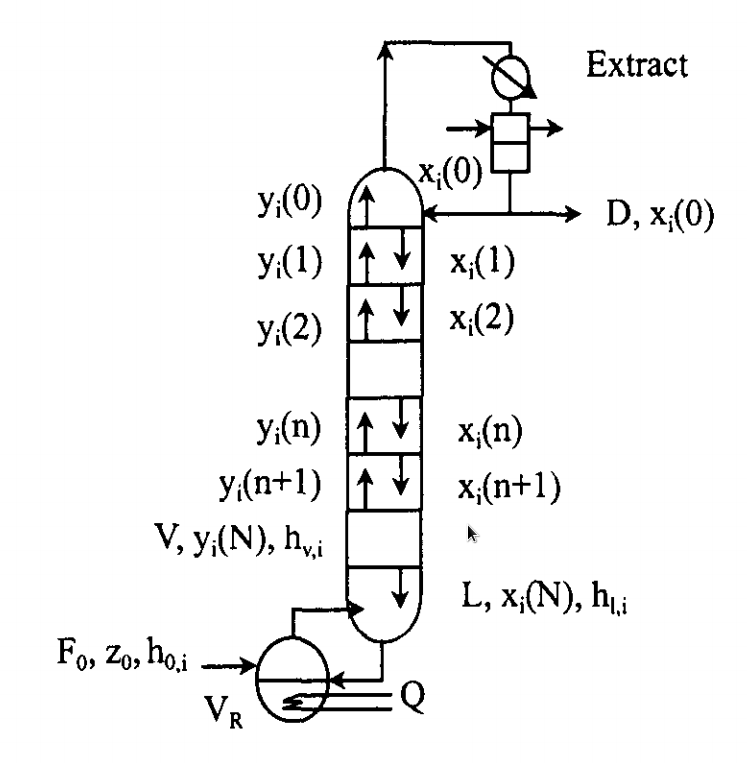
\includegraphics[scale=0.45]{img/reaccol.png}
 \caption{ The coupled reactor/column system (adapted from \citet{HU19991353}).} \label{fig:col}
\end{figure}
 
The feed stream of the reactor contains an aqueous solution of formaldehyde and water.
The goal of the process is to maximise the overall conversion of formaldehyde to trioxane.

\section{Model}
% % Assumptions
The following assumptions have been made for the process.
\begin{enumerate}
\item The entire reactor/column system operates at a continuous steady state equilibrium.
\item The reactor is controlled at a set temperature and the heat transfer dynamics is negligible.
\item The system is adiabatic so that no heat is lost to the environment.
\item The catalytic reaction occurs in the liquid phase of the reactor only. No reaction occurs in the column equilibrium stages.
\item Side reactions and intermediate products are negligible so that the system is a tertiary formaldyhyde-trioxane-water system.
\item A constant relatively volatility is assumed at all stages of the reaction.
\end{enumerate}

The system equations as developed by \citet{HU19991353} are shown in \autoref{tab:equations2}. %A description of parameter, input and output variable names as well as initial steady-state values are presented in Tables~\ref{tab:parameters},~\ref{tab:inputs} and~\ref{tab:outputs}.

%\include{solution_steps}

\begin{landscape}
\begin{table}[htbp]
  \centering
  \caption{System equations. Here $i$ is the chemical component index where $i = 1$ is formaldehyde, $i = 2$  is trioxane and $i=3$ is water. $n$ represents an equilibrium stage $n = 0, 1, 2, \dots N$, the stage $n = N$ is the reactor stage.}
  \label{tab:equations2}
  \begin{tabular}{rllll}
    \toprule
                                  & Equation                                            
                                  & Parameters          
                                  & Inputs         
                                  & Outputs  \\
    \midrule
    \describesection{Reactor mass balance} \\
    \eq                           & $F z_{i} + L x_{i, N} - V y_{i, N} + \upsilon_i r = 0$                           
                                  &   \defparameter{\upsilon_i}
                                  & \definput{F}  \definput{z_{i}}
                                  & \defoutput{ x_{i, N}  }   \defoutput{  y_{i, N}   }  \defoutput{ L }  \defoutput{ V }  \defoutput{  r}    \\
    \describesection{Column mass balance} \\
    \eq                           & $V y_{i, n} - (L + w_i D) x_{i, n} = 0$    
                                  &   \defparameter{w_i}
                                  & \definput{D}
                                  & \defoutput{x_{i, n}}  \defoutput{y_{i, n}} \\
    \eq                           & $L = R D$    
                                  &                       
                                  & \definput{R}
                                  & \\
    \describesection{Component continuity} \\
    \eq                           & $\sum^3_i z_{i} = 1$    
                                  &                       
                                  & 
                                  & \\
    \eq                           & $\sum^3_i x_{i,n} = 1$    
                                  &                       
                                  & 
                                  & \\
    \eq                           & $\sum^3_i y_{i,n} = 1$    
                                  &                       
                                  & 
                                  & \\
    \describesection{Phase equilibrium} \\
    \eq                           & $ \alpha_i = \frac{ y_{i,n} / y_{1, n} }{ x_{i, n+1} / x_{_{1, n + 1}} } $    
                                  &                       
                                  & 
                                  & \defoutput{\alpha_i} \\
    \describesection{Reaction rate equation} \\
    \eq                           & $ r = V_r \left( k_1 C_1^2 - k_2 C_2 \right)  $    
                                  &  \defparameter{k_1} \defparameter{k_2}       
                                  & 
                                  & \defoutput{r}\\
    \describesection{Energy balance} \\
    \eq                           & $ \sum^3_i \left[ Fz_i h_{F, i} + L x_{i, N} h_{l, i} - V y_{i, N} h_{v, i} \right] + Q = 0$    
                                 &                       
                                  & \definput{ h_{F, i} } \definput{ h_{l, i} } \definput{ h_{v, i} } \definput{ Q }
                                 & \\
    \midrule
                                  & Total: \arabic{variables} = & \arabic{parameters} & +\arabic{inputs} & +\arabic{outputs}  \\
    \bottomrule
  \end{tabular}
\end{table}

\end{landscape}



\section{Instructions}

Based on your findings from the initial investigation into the process model it was decided that a more sophisticated thermodynamic model would be required to accurately simulate this system. It was decided to incorporate a cubic equation of state into the model. To calculate the fugacities from the mechanical equation of state (a PVT relation) we will need to find expressions for the fugacity coefficient of a component in a mixture.

The Peng-Robinson equation of state is given by
$$
P = \frac{RT}{v - b} - \frac{a}{ v(v + b) + b (v - b)}
$$

The fugacity coefficient of a component $i$ in a mixture can be calculated using Equation 11.60 from Smith, Van Ness and Abbott (SvA) p. 404
$$
\ln{\hat{\phi}_i} = \int^P_0 (\bar{Z}_i - 1) \frac{d P}{P}
$$
where $\bar{Z}_i  = \frac{\left( \partial n Z \right)}{\partial n_i}$. Using this equation together with the Van der Waals mixing parameters. (SvA Equations 14.42 and 14.43 p. 561)
$$
b = \sum_{i} x_i b_i
$$

$$
a = \sum_{i}\sum_{j} x_i x_j a_{ij}
$$
 where $a_{ij} = \sqrt{a_i a_j}$
 

%%PR


 Show that the fugacity coefficient of component $i$ in a mixture described by the Peng-Robinson equation of state is given by
 
$$
\ln{\hat{\phi}_i} = \frac{b_i}{b} (z - 1) - \ln{\left( Z - \frac{b P}{RT} \right) - \frac{a}{2 \sqrt{2} b R T} \left(\frac{2 \sum_{j} y_j a_{ij}}{a} - \frac{b_i}{b} \right) \ln{\left( \frac{ v + b \left( 1 + \sqrt{2}\right) }{v + b \left( 1 - \sqrt{2}\right) }\right)}}
$$ 

 
\begin{centering}
Total Marks: \Ovalbox{100}\\
\end{centering}

%\pagebreak
\bibliographystyle{apalike}
%\bibliographystyle{spmpsci}
\bibliography{lib}


\end{document}
